\documentclass{article}

\usepackage{wrapstuff}
\usepackage{graphicx}
\usepackage{caption}

\usepackage[fontsize=14pt]{fontsize}
\usepackage{fontspec}
\setmainfont{CMU Serif}
\setmonofont{CMU Typewriter Text}
\defaultfontfeatures{Ligatures={TeX}}
\usepackage[english, ukrainian]{babel}
\usepackage{microtype}

\usepackage[
	a4paper,
	footskip=1cm,
	headsep=0.3cm,
	top=2cm,
	bottom=2cm,
	left=2cm,
	right=2cm
    ]{geometry}

\graphicspath{{Pictures}}

\begin{document}
\thispagestyle{empty}

\begin{wrapstuff}[type=figure, width=0.4\textwidth, l,top=4]
	\centering
	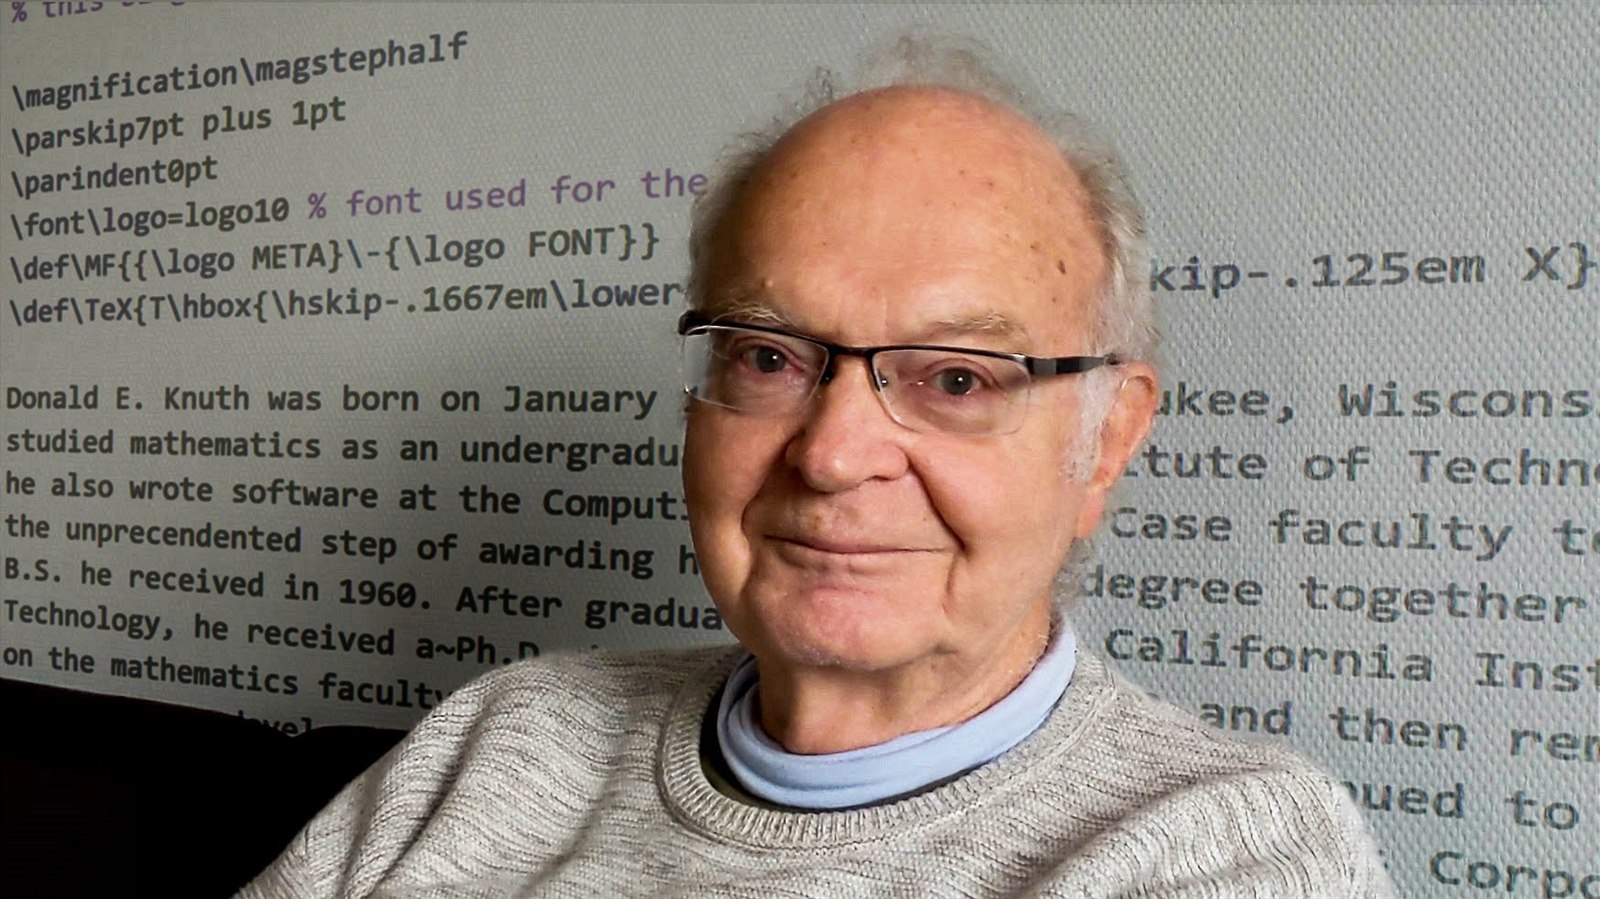
\includegraphics[width=\linewidth]{Knuth}
	\caption{Дональд Ервін Кнут}
	\label{pic: Knuth}
\end{wrapstuff}


Дональд Ервін Кнут (рис.~\ref{pic: Knuth}) (10 січня 1938 , Мілвокі, Вісконсин ) --- інформатик, ідеолог програмування та почесний професор Стенфордського університету. Автор фундаментальної праці \textit{«Мистецтво програмування»}; вважається одним з батьків аналізу складності алгоритмів. Розробник типографічної системи \TeX{} та пов'язаної мови визначення шрифтів і системи їх рендерингу \texttt{METAFONT}.

Кнут народився у місті Мілвокі, штат Вісконсин, в сім'ї німецьких американців Генрі Кнута та Луізи Марії Бонінг. Батько Дональда працював на двох роботах: викладав бухгалетерію у Старшій Школі Мілвокі та вів невелике підприємство по друку. Молодший Кнут, навчаючись у тій же школі, отримав багато академічних відзнак, більшість з яких за геніальні способи вирішення різноманітних проблем. Наприклад, у восьмому класі він взяв участь у змаганні, в якому потрібно було відшукати всі слова, які можна скласти з букв словосполуки «Ziegler's Giant Bar». У суддейському списку було 2500 слів, та Дональду вдалось знайти 4500 та перемогти у конкурсі.

Освіта У 1956 році Кнут отримав запрошення до Технологічного Інституту (рис.~\ref{pic: CWRU}) у Клівленді, Огайо, де вперше познайомився з \texttt{IBM} 650, одним із перших мейнфреймів. Прочитавши посібник до комп'ютера, Кнут вирішив переписати код компілятора для комп'ютера з його колишньої школи, тому що
він вірив, що зможе зробити його краще.

\begin{figure}[h!]
	\hfill\hfill\hfill
	\begin{minipage}[c]{0.5\textwidth}
		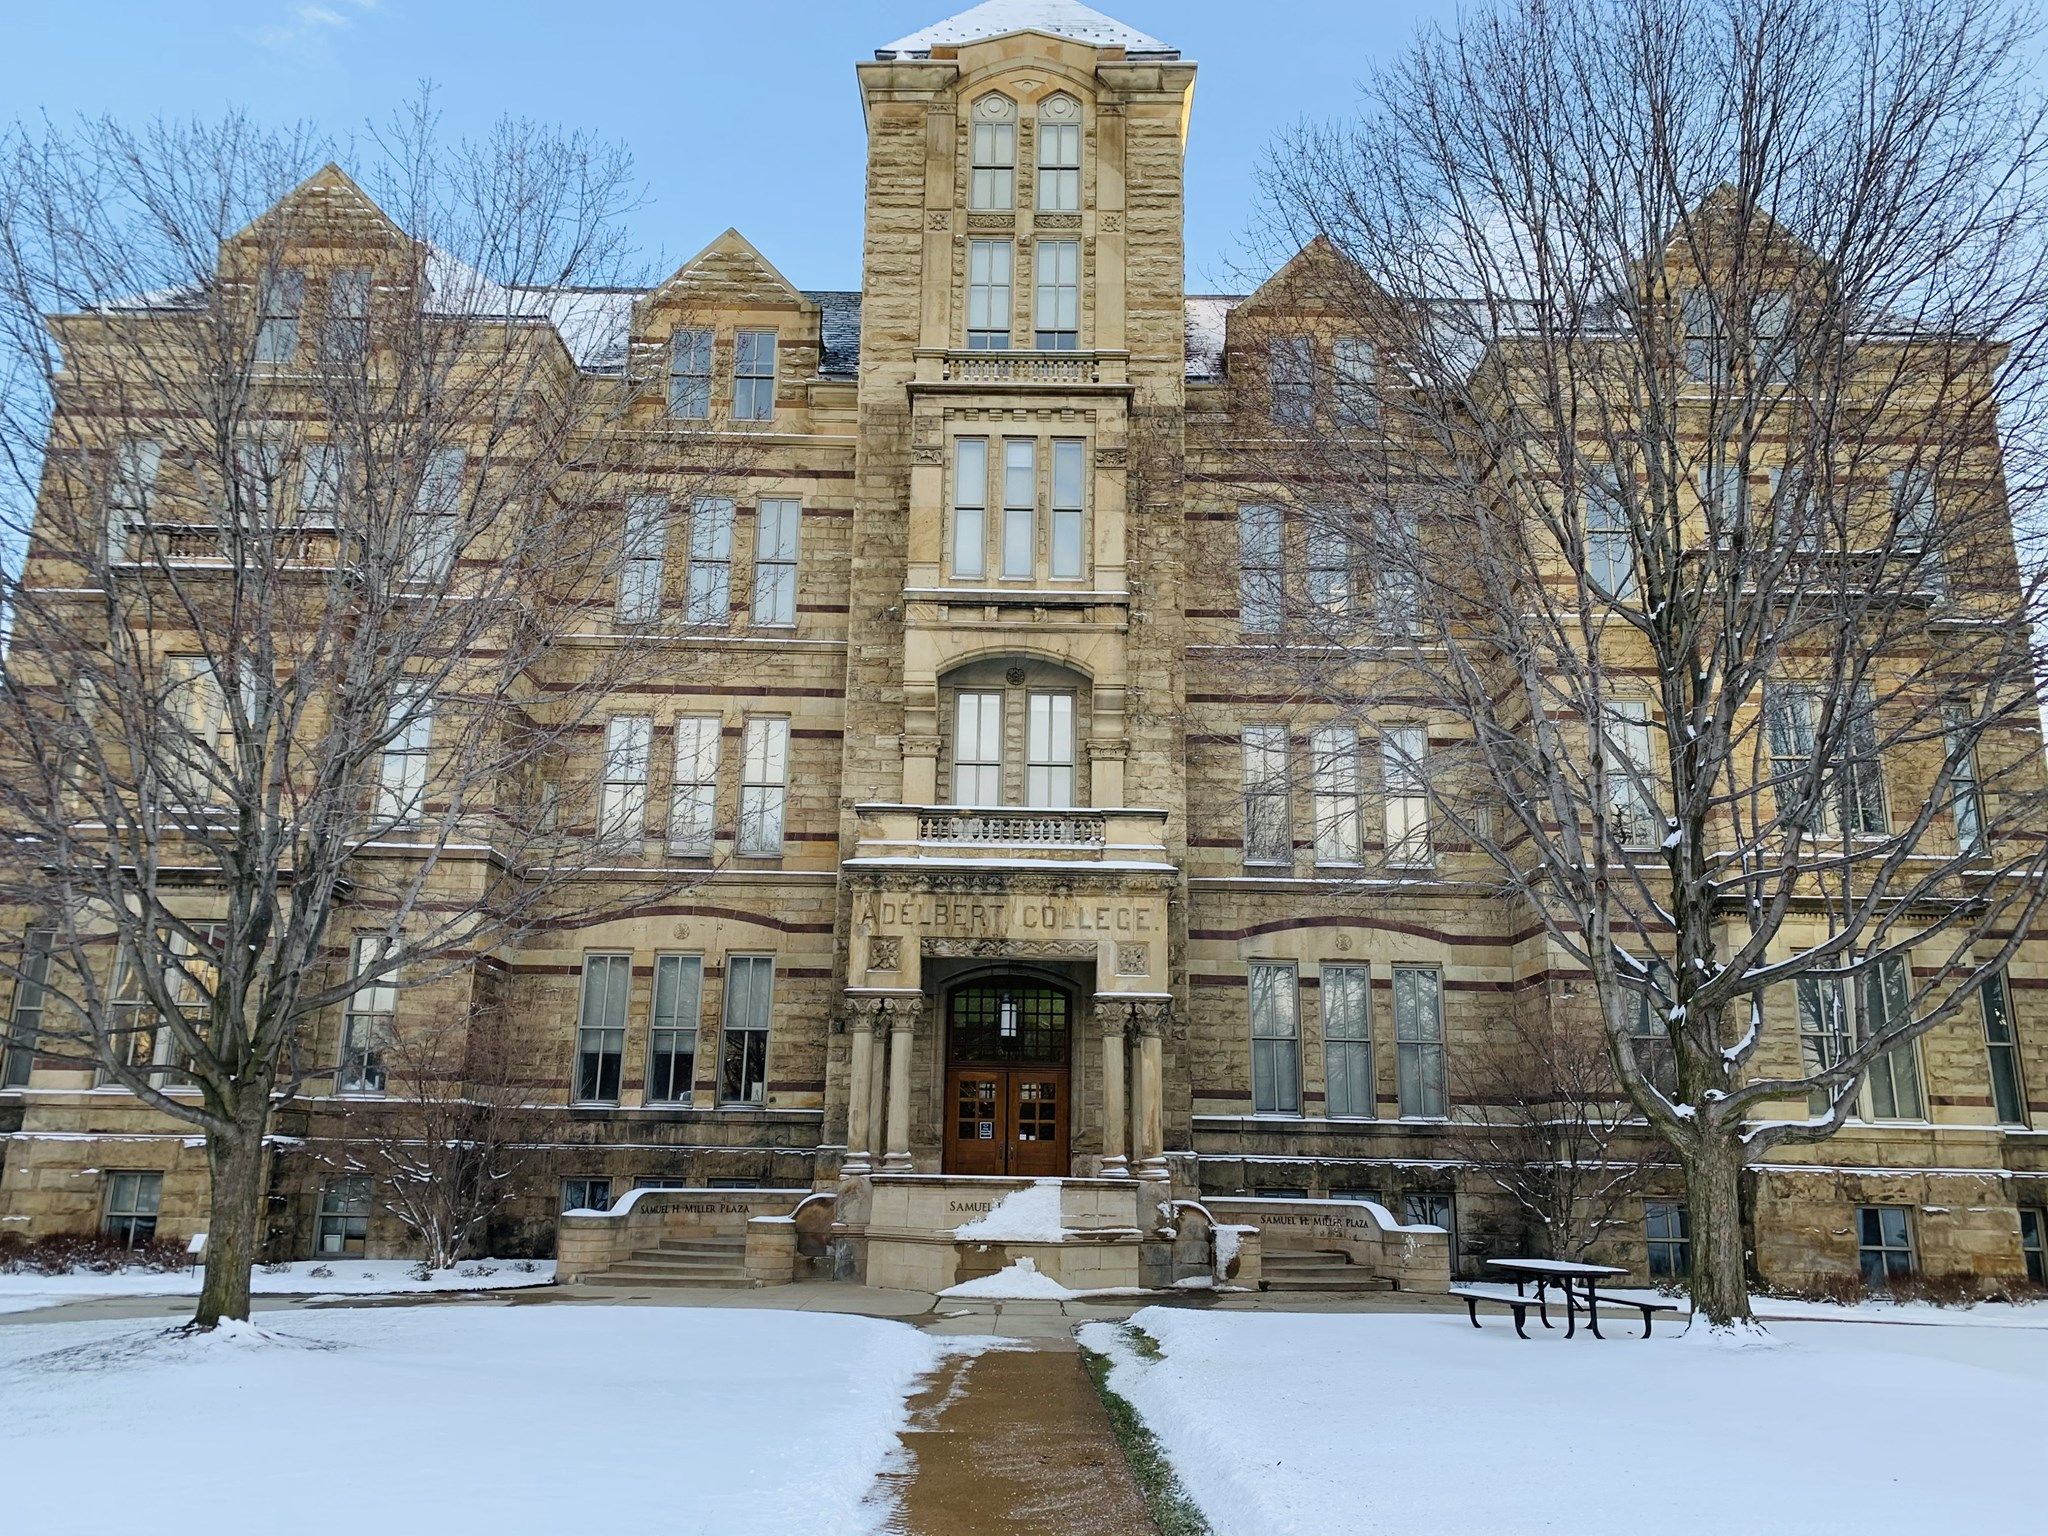
\includegraphics[width=\linewidth]{CWRU}
	\end{minipage}
	\hfill
	\begin{minipage}[c]{0.38\textwidth}
		\caption{Західний резервний\\університет Кейса (CWRU)}
		\label{pic: CWRU}
	\end{minipage}
	\hfill\hfill\hfill
\end{figure}

У 1958 році Кнут створив програму, щоб допомогти шкільній баскетбольній команді вигравати більше матчів. Він призначив кожному гравцю
«вартість», щоб оцінити імовірність кожного баскетболіста здобути очки. Цей підхід оцінили видання Newsweek і CBS Evening News, згадавши Кнута
у своїх випусках.
\end{document}